% Options for packages loaded elsewhere
\PassOptionsToPackage{unicode}{hyperref}
\PassOptionsToPackage{hyphens}{url}
%
\documentclass[
]{article}
\usepackage{amsmath,amssymb}
\usepackage{lmodern}
\usepackage{iftex}
\ifPDFTeX
  \usepackage[T1]{fontenc}
  \usepackage[utf8]{inputenc}
  \usepackage{textcomp} % provide euro and other symbols
\else % if luatex or xetex
  \usepackage{unicode-math}
  \defaultfontfeatures{Scale=MatchLowercase}
  \defaultfontfeatures[\rmfamily]{Ligatures=TeX,Scale=1}
\fi
% Use upquote if available, for straight quotes in verbatim environments
\IfFileExists{upquote.sty}{\usepackage{upquote}}{}
\IfFileExists{microtype.sty}{% use microtype if available
  \usepackage[]{microtype}
  \UseMicrotypeSet[protrusion]{basicmath} % disable protrusion for tt fonts
}{}
\makeatletter
\@ifundefined{KOMAClassName}{% if non-KOMA class
  \IfFileExists{parskip.sty}{%
    \usepackage{parskip}
  }{% else
    \setlength{\parindent}{0pt}
    \setlength{\parskip}{6pt plus 2pt minus 1pt}}
}{% if KOMA class
  \KOMAoptions{parskip=half}}
\makeatother
\usepackage{xcolor}
\usepackage[margin=1in]{geometry}
\usepackage{color}
\usepackage{fancyvrb}
\newcommand{\VerbBar}{|}
\newcommand{\VERB}{\Verb[commandchars=\\\{\}]}
\DefineVerbatimEnvironment{Highlighting}{Verbatim}{commandchars=\\\{\}}
% Add ',fontsize=\small' for more characters per line
\usepackage{framed}
\definecolor{shadecolor}{RGB}{248,248,248}
\newenvironment{Shaded}{\begin{snugshade}}{\end{snugshade}}
\newcommand{\AlertTok}[1]{\textcolor[rgb]{0.94,0.16,0.16}{#1}}
\newcommand{\AnnotationTok}[1]{\textcolor[rgb]{0.56,0.35,0.01}{\textbf{\textit{#1}}}}
\newcommand{\AttributeTok}[1]{\textcolor[rgb]{0.77,0.63,0.00}{#1}}
\newcommand{\BaseNTok}[1]{\textcolor[rgb]{0.00,0.00,0.81}{#1}}
\newcommand{\BuiltInTok}[1]{#1}
\newcommand{\CharTok}[1]{\textcolor[rgb]{0.31,0.60,0.02}{#1}}
\newcommand{\CommentTok}[1]{\textcolor[rgb]{0.56,0.35,0.01}{\textit{#1}}}
\newcommand{\CommentVarTok}[1]{\textcolor[rgb]{0.56,0.35,0.01}{\textbf{\textit{#1}}}}
\newcommand{\ConstantTok}[1]{\textcolor[rgb]{0.00,0.00,0.00}{#1}}
\newcommand{\ControlFlowTok}[1]{\textcolor[rgb]{0.13,0.29,0.53}{\textbf{#1}}}
\newcommand{\DataTypeTok}[1]{\textcolor[rgb]{0.13,0.29,0.53}{#1}}
\newcommand{\DecValTok}[1]{\textcolor[rgb]{0.00,0.00,0.81}{#1}}
\newcommand{\DocumentationTok}[1]{\textcolor[rgb]{0.56,0.35,0.01}{\textbf{\textit{#1}}}}
\newcommand{\ErrorTok}[1]{\textcolor[rgb]{0.64,0.00,0.00}{\textbf{#1}}}
\newcommand{\ExtensionTok}[1]{#1}
\newcommand{\FloatTok}[1]{\textcolor[rgb]{0.00,0.00,0.81}{#1}}
\newcommand{\FunctionTok}[1]{\textcolor[rgb]{0.00,0.00,0.00}{#1}}
\newcommand{\ImportTok}[1]{#1}
\newcommand{\InformationTok}[1]{\textcolor[rgb]{0.56,0.35,0.01}{\textbf{\textit{#1}}}}
\newcommand{\KeywordTok}[1]{\textcolor[rgb]{0.13,0.29,0.53}{\textbf{#1}}}
\newcommand{\NormalTok}[1]{#1}
\newcommand{\OperatorTok}[1]{\textcolor[rgb]{0.81,0.36,0.00}{\textbf{#1}}}
\newcommand{\OtherTok}[1]{\textcolor[rgb]{0.56,0.35,0.01}{#1}}
\newcommand{\PreprocessorTok}[1]{\textcolor[rgb]{0.56,0.35,0.01}{\textit{#1}}}
\newcommand{\RegionMarkerTok}[1]{#1}
\newcommand{\SpecialCharTok}[1]{\textcolor[rgb]{0.00,0.00,0.00}{#1}}
\newcommand{\SpecialStringTok}[1]{\textcolor[rgb]{0.31,0.60,0.02}{#1}}
\newcommand{\StringTok}[1]{\textcolor[rgb]{0.31,0.60,0.02}{#1}}
\newcommand{\VariableTok}[1]{\textcolor[rgb]{0.00,0.00,0.00}{#1}}
\newcommand{\VerbatimStringTok}[1]{\textcolor[rgb]{0.31,0.60,0.02}{#1}}
\newcommand{\WarningTok}[1]{\textcolor[rgb]{0.56,0.35,0.01}{\textbf{\textit{#1}}}}
\usepackage{longtable,booktabs,array}
\usepackage{calc} % for calculating minipage widths
% Correct order of tables after \paragraph or \subparagraph
\usepackage{etoolbox}
\makeatletter
\patchcmd\longtable{\par}{\if@noskipsec\mbox{}\fi\par}{}{}
\makeatother
% Allow footnotes in longtable head/foot
\IfFileExists{footnotehyper.sty}{\usepackage{footnotehyper}}{\usepackage{footnote}}
\makesavenoteenv{longtable}
\usepackage{graphicx}
\makeatletter
\def\maxwidth{\ifdim\Gin@nat@width>\linewidth\linewidth\else\Gin@nat@width\fi}
\def\maxheight{\ifdim\Gin@nat@height>\textheight\textheight\else\Gin@nat@height\fi}
\makeatother
% Scale images if necessary, so that they will not overflow the page
% margins by default, and it is still possible to overwrite the defaults
% using explicit options in \includegraphics[width, height, ...]{}
\setkeys{Gin}{width=\maxwidth,height=\maxheight,keepaspectratio}
% Set default figure placement to htbp
\makeatletter
\def\fps@figure{htbp}
\makeatother
\setlength{\emergencystretch}{3em} % prevent overfull lines
\providecommand{\tightlist}{%
  \setlength{\itemsep}{0pt}\setlength{\parskip}{0pt}}
\setcounter{secnumdepth}{-\maxdimen} % remove section numbering
\ifLuaTeX
  \usepackage{selnolig}  % disable illegal ligatures
\fi
\IfFileExists{bookmark.sty}{\usepackage{bookmark}}{\usepackage{hyperref}}
\IfFileExists{xurl.sty}{\usepackage{xurl}}{} % add URL line breaks if available
\urlstyle{same} % disable monospaced font for URLs
\hypersetup{
  pdftitle={Heart diseases feature selection and exploratory data analysis},
  pdfauthor={Wangjun Shen},
  hidelinks,
  pdfcreator={LaTeX via pandoc}}

\title{Heart diseases feature selection and exploratory data analysis}
\author{Wangjun Shen}
\date{}

\begin{document}
\maketitle

\hypertarget{introduction}{%
\section{Introduction}\label{introduction}}

The objective of this assignment is to prepare a data set that can be
used to predict heart disease, a common and serious health issue that
affects a significant portion of the population. The data set we will be
working on is a subset of a larger real-world data set collected by
multiple healthcare institutions. It contains various attributes related
to patients' health, such as age, gender, blood pressure, and other
clinical measurements. These attributes can be leveraged to predict the
presence of heart disease.

Data mining plays a critical role in addressing challenges related to
predicting disease spread and similar healthcare problems. By analyzing
large and complex data sets, we can identify patterns and relationships
that may not be immediately apparent. This, in turn, allows us to
develop more accurate predictive models. In the context of heart
disease, data mining techniques can help us extract insights and
patterns from patient data. These insights can aid in identifying risk
factors, predicting disease outcomes, and developing effective treatment
strategies.

For example, by using data mining techniques on the given data set, we
can identify the most important predictors of heart disease. This
knowledge can then be used to develop a classification model that
accurately predicts the presence of the disease in patients. Moreover,
data mining can also help us identify subpopulations that are more
susceptible to the disease. We can then develop tailored prevention and
treatment strategies for these subpopulations.

Overall, this assignment provides an opportunity to apply data mining
techniques to a real-world data set. It also allows us to gain hands-on
experience with feature engineering, data exploration, and predictive
modeling. The insights gained from this exploration can inform our work
in subsequent assignments. This, in turn, can help us develop more
accurate and effective predictive models for heart disease and other
similar health challenges.

\hypertarget{related-work}{%
\section{Related Work}\label{related-work}}

\begin{center}\rule{0.5\linewidth}{0.5pt}\end{center}

\hypertarget{data-exploration}{%
\section{Data exploration}\label{data-exploration}}

\hypertarget{features-selection}{%
\subsection{Features Selection}\label{features-selection}}

The details of the original data set are as follows.

\begin{longtable}[]{@{}
  >{\raggedright\arraybackslash}p{(\columnwidth - 4\tabcolsep) * \real{0.3333}}
  >{\raggedright\arraybackslash}p{(\columnwidth - 4\tabcolsep) * \real{0.3333}}
  >{\raggedright\arraybackslash}p{(\columnwidth - 4\tabcolsep) * \real{0.3333}}@{}}
\toprule()
\begin{minipage}[b]{\linewidth}\raggedright
Variable
\end{minipage} & \begin{minipage}[b]{\linewidth}\raggedright
Description
\end{minipage} & \begin{minipage}[b]{\linewidth}\raggedright
Type
\end{minipage} \\
\midrule()
\endhead
id & A unique ID that identifies a participant in the study &
Numerical \\
age & Age in years & Numerical \\
sex & Male and Female were recorded & Categorical \\
cp & Chest Pain type: typical angina; atypical angina; non-anginal pain;
and asymptomatic & Categorical \\
trestbps & Resting blood pressure (in mm Hg on admission to the
hospital) & Numerical \\
chol & Serum Cholestoral in mg/dl & Numerical \\
fbs & Fasting blood sugar \textgreater{} 120 mg/dl (True or False) &
Boolean \\
restecg & Resting electrocardiographic results: normal; having ST-T wave
abnormality (T wave inversions and/or ST elevation or depression of
\textgreater{} 0.05 mV) or showing probable or definite left ventricular
hypertrophy by Estes' criteria & Categorical \\
thalach & Maximum heart rate achieved & Numerical \\
exang & Exercise induced angina (True/False) & Boolean \\
oldpeak & ST depression induced by exercise relative to rest &
Numerical \\
slope & The slope of the peak exercise ST segment: upsloping; flat;
downsloping & Categorical \\
major\_vessels & Number of major vessels (0-3) colored by flourosopy &
Numerical \\
restwm & Rest wall motion abnormality: none; mild or moderate; moderate
or severe; akinesis or dyskmem & Categorical \\
target & Heart disease diagnosed (disease/no disease) & Categorical \\
\bottomrule()
\end{longtable}

Import the data set and view.

\begin{Shaded}
\begin{Highlighting}[]
\CommentTok{\# load data set first}
\NormalTok{heart.full }\OtherTok{\textless{}{-}} \FunctionTok{read.csv}\NormalTok{(}\StringTok{"heart.csv"}\NormalTok{)}

\CommentTok{\# then check the data set}
\FunctionTok{str}\NormalTok{(heart.full)}
\end{Highlighting}
\end{Shaded}

\begin{verbatim}
## 'data.frame':    1025 obs. of  15 variables:
##  $ id           : int  1 2 3 4 5 6 7 8 9 10 ...
##  $ age          : int  52 53 70 61 62 58 58 55 46 54 ...
##  $ sex          : chr  "male" "male" "male" "male" ...
##  $ cp           : chr  "typical angina" "typical angina" "typical angina" "typical angina" ...
##  $ trestbps     : int  125 140 145 148 138 100 114 160 120 122 ...
##  $ chol         : int  212 203 174 203 294 248 318 289 249 286 ...
##  $ fbs          : logi  FALSE TRUE FALSE FALSE TRUE FALSE ...
##  $ restecg      : chr  "ST-T wave abnormality" "normal" "ST-T wave abnormality" "ST-T wave abnormality" ...
##  $ thalach      : int  168 155 125 161 106 122 140 145 144 116 ...
##  $ exang        : logi  FALSE TRUE TRUE FALSE FALSE FALSE ...
##  $ oldpeak      : num  1 3.1 2.6 0 1.9 1 4.4 0.8 0.8 3.2 ...
##  $ slope        : chr  "downsloping" "upsloping" "upsloping" "downsloping" ...
##  $ major_vessels: int  2 0 0 1 3 0 3 1 0 2 ...
##  $ restwm       : chr  "akinesis or dyskmem" "akinesis or dyskmem" "akinesis or dyskmem" "akinesis or dyskmem" ...
##  $ target       : chr  "no disease" "no disease" "no disease" "no disease" ...
\end{verbatim}

From the output results, it can be found that the data set contains 15
variables and 1025 observation. The details of each variable are
consistent with the description.

Then check the distribution of missing values in the data set.

\begin{Shaded}
\begin{Highlighting}[]
\FunctionTok{sum}\NormalTok{(}\FunctionTok{is.na}\NormalTok{(heart.full))}
\end{Highlighting}
\end{Shaded}

\begin{verbatim}
## [1] 0
\end{verbatim}

There are not missing values in this data.

In the following section, we will discuss the importance of features,
specifically the correlation between variables. To measure this
correlation, we will use random forest to calculate Gini Importance or
Mean Decrease in Impurity (MDI). This method determines the importance
of each feature by summing the number of splits (across all trees) that
include the feature, proportionally to the number of samples it splits.

The first is the correlation coefficient between the variables. The data
set is undergoing a transformation from its original data types to
appropriate data types required for analysis. Originally, the variables
age, trestbps, chol, thalach, and oldpeak were imported as character
vectors representing age, resting blood pressure, serum cholesterol,
maximum heart rate achieved, and ST depression induced by exercise
relative to rest, respectively. These variables have been converted to a
numeric data type since they represent numerical measurements.
Similarly, the variables sex, cp, restecg, slope, restwm, and target
were originally imported as character vectors representing sex, chest
pain type, resting electrocardiographic results, slope of the peak
exercise ST segment, presence of a major vessels colored by fluoroscopy,
and heart disease status, respectively. These variables have been
converted to factor data type since they represent categorical
variables. This transformation allows for easier data manipulation and
analysis, especially when exploring relationships between variables.

\begin{Shaded}
\begin{Highlighting}[]
\CommentTok{\# convert age, trestbps, chol, thalach, and oldpeak to numeric}
\NormalTok{heart.full}\SpecialCharTok{$}\NormalTok{age }\OtherTok{\textless{}{-}} \FunctionTok{as.numeric}\NormalTok{(heart.full}\SpecialCharTok{$}\NormalTok{age)}
\NormalTok{heart.full}\SpecialCharTok{$}\NormalTok{trestbps }\OtherTok{\textless{}{-}} \FunctionTok{as.numeric}\NormalTok{(heart.full}\SpecialCharTok{$}\NormalTok{trestbps)}
\NormalTok{heart.full}\SpecialCharTok{$}\NormalTok{chol }\OtherTok{\textless{}{-}} \FunctionTok{as.numeric}\NormalTok{(heart.full}\SpecialCharTok{$}\NormalTok{chol)}
\NormalTok{heart.full}\SpecialCharTok{$}\NormalTok{thalach }\OtherTok{\textless{}{-}} \FunctionTok{as.numeric}\NormalTok{(heart.full}\SpecialCharTok{$}\NormalTok{thalach)}
\NormalTok{heart.full}\SpecialCharTok{$}\NormalTok{oldpeak }\OtherTok{\textless{}{-}} \FunctionTok{as.numeric}\NormalTok{(heart.full}\SpecialCharTok{$}\NormalTok{oldpeak)}


\CommentTok{\# }
\CommentTok{\# heart.full$sex \textless{}{-} as.numeric(heart.full$sex)}
\CommentTok{\# heart.full$cp \textless{}{-} as.numeric(heart.full$cp)}
\CommentTok{\# heart.full$restecg \textless{}{-} as.numeric(heart.full$restecg)}
\CommentTok{\# heart.full$slope \textless{}{-} as.numeric(heart.full$slope)}
\CommentTok{\# heart.full$restwm \textless{}{-} as.numeric(heart.full$restwm)}
\CommentTok{\# heart.full$target \textless{}{-} as.numeric(heart.full$target)}

\CommentTok{\# }
\CommentTok{\# convert sex, cp, restecg, slope, restwm, and target to factor}
\NormalTok{heart.full}\SpecialCharTok{$}\NormalTok{sex }\OtherTok{\textless{}{-}} \FunctionTok{as.factor}\NormalTok{(heart.full}\SpecialCharTok{$}\NormalTok{sex)}
\NormalTok{heart.full}\SpecialCharTok{$}\NormalTok{cp }\OtherTok{\textless{}{-}} \FunctionTok{as.factor}\NormalTok{(heart.full}\SpecialCharTok{$}\NormalTok{cp)}
\NormalTok{heart.full}\SpecialCharTok{$}\NormalTok{restecg }\OtherTok{\textless{}{-}} \FunctionTok{as.factor}\NormalTok{(heart.full}\SpecialCharTok{$}\NormalTok{restecg)}
\NormalTok{heart.full}\SpecialCharTok{$}\NormalTok{slope }\OtherTok{\textless{}{-}} \FunctionTok{as.factor}\NormalTok{(heart.full}\SpecialCharTok{$}\NormalTok{slope)}
\NormalTok{heart.full}\SpecialCharTok{$}\NormalTok{restwm }\OtherTok{\textless{}{-}} \FunctionTok{as.factor}\NormalTok{(heart.full}\SpecialCharTok{$}\NormalTok{restwm)}
\NormalTok{heart.full}\SpecialCharTok{$}\NormalTok{target }\OtherTok{\textless{}{-}} \FunctionTok{as.factor}\NormalTok{(heart.full}\SpecialCharTok{$}\NormalTok{target)}
\end{Highlighting}
\end{Shaded}

Next we calculate the correlation between the variables.

\begin{Shaded}
\begin{Highlighting}[]
\CommentTok{\# calculate the correlation matrix}
\CommentTok{\# if convert to factor}
\NormalTok{cor.matrix }\OtherTok{\textless{}{-}} \FunctionTok{cor}\NormalTok{(heart.full[, }\FunctionTok{c}\NormalTok{(}\StringTok{"age"}\NormalTok{, }\StringTok{"trestbps"}\NormalTok{, }\StringTok{"chol"}\NormalTok{, }\StringTok{"thalach"}\NormalTok{, }\StringTok{"oldpeak"}\NormalTok{, }\StringTok{"major\_vessels"}\NormalTok{)])}
\NormalTok{cor.matrix}
\end{Highlighting}
\end{Shaded}

\begin{verbatim}
##                      age    trestbps        chol     thalach     oldpeak
## age            1.0000000  0.27112141  0.21982253 -0.39022708  0.20813668
## trestbps       0.2711214  1.00000000  0.12797743 -0.03926407  0.18743411
## chol           0.2198225  0.12797743  1.00000000 -0.02177209  0.06488031
## thalach       -0.3902271 -0.03926407 -0.02177209  1.00000000 -0.34979616
## oldpeak        0.2081367  0.18743411  0.06488031 -0.34979616  1.00000000
## major_vessels  0.2715505  0.10455372  0.07425934 -0.20788842  0.22181603
##               major_vessels
## age              0.27155053
## trestbps         0.10455372
## chol             0.07425934
## thalach         -0.20788842
## oldpeak          0.22181603
## major_vessels    1.00000000
\end{verbatim}

\begin{Shaded}
\begin{Highlighting}[]
\CommentTok{\# if convert to numeric}
\CommentTok{\# cor.matrix.numeric \textless{}{-} cor(heart.full)}
\CommentTok{\# cor.matrix.numeric}
\end{Highlighting}
\end{Shaded}

For ease of observation, we visualize the correlation.

\begin{Shaded}
\begin{Highlighting}[]
\FunctionTok{library}\NormalTok{(corrplot)}
\end{Highlighting}
\end{Shaded}

\begin{verbatim}
## Warning: package 'corrplot' was built under R version 4.2.3
\end{verbatim}

\begin{verbatim}
## corrplot 0.92 loaded
\end{verbatim}

\begin{Shaded}
\begin{Highlighting}[]
\FunctionTok{corrplot}\NormalTok{(cor.matrix, }\AttributeTok{method =} \StringTok{"color"}\NormalTok{)}
\end{Highlighting}
\end{Shaded}

\begin{figure}
\centering
\includegraphics{heart_eda_files/figure-latex/gg-oz-gapminder-1.pdf}
\caption{Visualization of correlation matrix}
\end{figure}

The resulting plot will show the correlations between variables using
different colors, where red indicates strong negative correlation, blue
indicates strong positive correlation, and white indicates no
correlation. The strength of the correlation is determined by the
absolute value of the correlation coefficient, with values closer to 1
indicating stronger correlation.

Then use random forest to detect the importance of each feature.In order
to understand whether these features differ between genders, the data
will firstly be created based on the sub-dataset.

\begin{Shaded}
\begin{Highlighting}[]
\CommentTok{\# data set for each gender}
\NormalTok{heart.male }\OtherTok{\textless{}{-}} \FunctionTok{subset}\NormalTok{(heart.full, sex }\SpecialCharTok{==} \StringTok{"male"}\NormalTok{)}
\NormalTok{heart.female }\OtherTok{\textless{}{-}} \FunctionTok{subset}\NormalTok{(heart.full, sex }\SpecialCharTok{==} \StringTok{"female"}\NormalTok{)}
\end{Highlighting}
\end{Shaded}

Then use those two sub datasets to build the random forest:

\begin{Shaded}
\begin{Highlighting}[]
\CommentTok{\# Random forest for male subset}
\FunctionTok{library}\NormalTok{(randomForest)}
\end{Highlighting}
\end{Shaded}

\begin{verbatim}
## Warning: package 'randomForest' was built under R version 4.2.2
\end{verbatim}

\begin{verbatim}
## randomForest 4.7-1.1
\end{verbatim}

\begin{verbatim}
## Type rfNews() to see new features/changes/bug fixes.
\end{verbatim}

\begin{Shaded}
\begin{Highlighting}[]
\FunctionTok{set.seed}\NormalTok{(}\DecValTok{123}\NormalTok{)}
\NormalTok{rf\_model\_male }\OtherTok{\textless{}{-}} \FunctionTok{randomForest}\NormalTok{(target }\SpecialCharTok{\textasciitilde{}}\NormalTok{ ., }\AttributeTok{data =}\NormalTok{ heart.male, }\AttributeTok{importance =} \ConstantTok{TRUE}\NormalTok{, }\AttributeTok{ntree =} \DecValTok{500}\NormalTok{)}
\FunctionTok{importance}\NormalTok{(rf\_model\_male)}
\end{Highlighting}
\end{Shaded}

\begin{verbatim}
##                 disease no disease MeanDecreaseAccuracy MeanDecreaseGini
## id             1.606825   3.213858             3.376221        11.154653
## age           33.928469  40.857084            42.838250        34.448119
## sex            0.000000   0.000000             0.000000         0.000000
## cp            38.745483  36.059468            41.121602        47.161819
## trestbps      33.903759  37.024285            41.751265        25.962476
## chol          34.122660  35.756098            39.121768        29.972875
## fbs           16.795603  16.203869            19.636756         3.761825
## restecg       19.083360  19.416802            21.509917         5.531215
## thalach       37.581333  37.899592            43.252118        51.572260
## exang         17.532815  19.401905            20.468760        11.933409
## oldpeak       32.589020  38.902000            40.817055        37.108368
## slope         24.318522  24.566740            27.686364        17.111266
## major_vessels 37.680805  40.115231            43.835239        42.184090
## restwm        31.201322  32.398437            34.984151        25.367047
\end{verbatim}

Based on the provided correlation matrix, the following features appear
to be the most important in predicting the presence of heart disease:

\begin{itemize}
\tightlist
\item
  cp (chest pain type)
\item
  thalach (maximum heart rate achieved)
\item
  major\_vessels (number of major vessels colored by fluoroscopy)
\item
  oldpeak (ST depression induced by exercise relative to rest)
\item
  trestbps (resting blood pressure)
\item
  age
\end{itemize}

These features have the highest correlation with the target variable
(disease/no disease), as well as high values for MeanDecreaseAccuracy
and MeanDecreaseGini, indicating that they are important predictors for
a machine learning model.

Chest pain type (cp) has the highest correlation with the target
variable and high values for both MeanDecreaseAccuracy and
MeanDecreaseGini, suggesting that it is a strong predictor for heart
disease. Maximum heart rate achieved (thalach) and the number of major
vessels colored by fluoroscopy (major\_vessels) also have high
correlations and values for MeanDecreaseAccuracy and MeanDecreaseGini,
making them strong predictors as well. ST depression induced by exercise
relative to rest (oldpeak) and resting blood pressure (trestbps) have
lower correlations but still have high values for MeanDecreaseAccuracy
and MeanDecreaseGini, indicating that they are important features in
predicting the presence of heart disease. Finally, age is also an
important feature as it has a moderate correlation with the target
variable and a relatively high value for MeanDecreaseAccuracy.

Overall, these six features can be considered the most important for
predicting the presence of heart disease for male in this dataset.

Visualization.

\begin{Shaded}
\begin{Highlighting}[]
\FunctionTok{varImpPlot}\NormalTok{(rf\_model\_male, }\AttributeTok{col =} \StringTok{"red"}\NormalTok{, }\AttributeTok{pch =} \DecValTok{20}\NormalTok{)}
\end{Highlighting}
\end{Shaded}

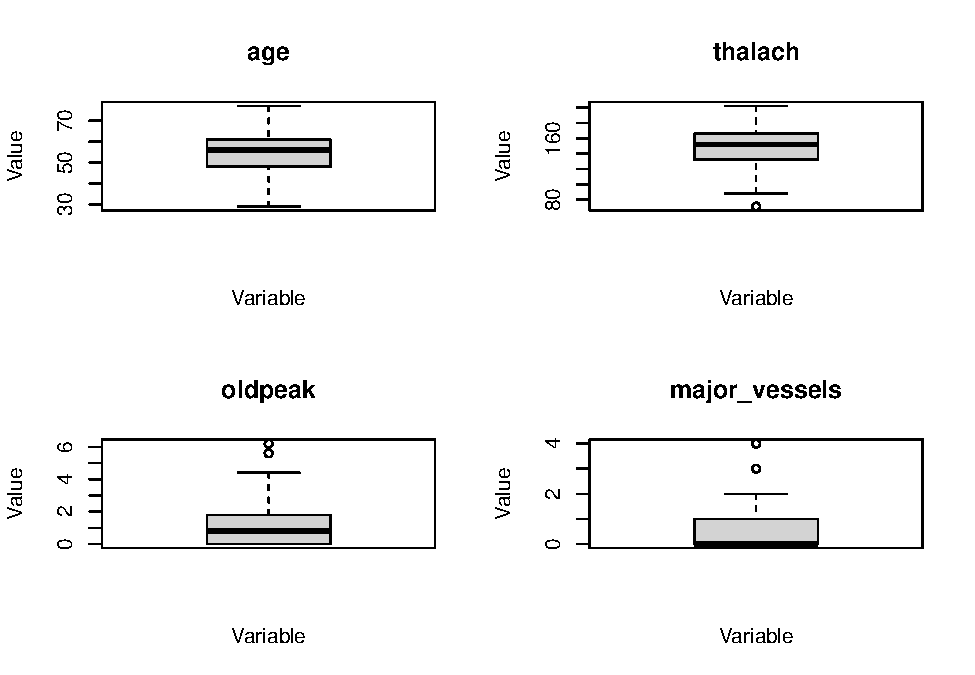
\includegraphics{heart_eda_files/figure-latex/unnamed-chunk-8-1.pdf}

\begin{Shaded}
\begin{Highlighting}[]
\CommentTok{\# Random forest for female subset}
\FunctionTok{set.seed}\NormalTok{(}\DecValTok{123}\NormalTok{)}
\NormalTok{rf\_model\_female }\OtherTok{\textless{}{-}} \FunctionTok{randomForest}\NormalTok{(target }\SpecialCharTok{\textasciitilde{}}\NormalTok{ ., }\AttributeTok{data =}\NormalTok{ heart.female, }\AttributeTok{importance =} \ConstantTok{TRUE}\NormalTok{, }\AttributeTok{ntree =} \DecValTok{500}\NormalTok{)}
\FunctionTok{importance}\NormalTok{(rf\_model\_female)}
\end{Highlighting}
\end{Shaded}

\begin{verbatim}
##                 disease no disease MeanDecreaseAccuracy MeanDecreaseGini
## id             1.932703  -3.148355           -0.5202009         2.590325
## age           23.376089  24.724758           28.2364781        12.018921
## sex            0.000000   0.000000            0.0000000         0.000000
## cp            19.702221  20.271296           22.9715941        12.537614
## trestbps      18.409296  18.651176           22.1370717         8.429236
## chol          19.941082  22.898914           25.6314494         8.321454
## fbs            7.611649   9.737944           10.2944996         1.418907
## restecg       14.299858  15.552097           17.3754050         2.982791
## thalach       19.430050  20.969639           24.2566433         8.272732
## exang         18.303884  21.574578           22.6248431         9.167964
## oldpeak       20.677704  21.784792           24.3639560        16.486048
## slope         17.218824  19.973871           21.5111294         8.150365
## major_vessels 19.573486  20.510840           22.7582749        10.407631
## restwm        22.156482  24.907233           26.5256308        22.290165
\end{verbatim}

Based on the provided correlation matrix, the important features that
can be selected are:

\begin{itemize}
\item
  Age: It has a high correlation with both disease and no disease, and
  also has high values for MeanDecreaseAccuracy and MeanDecreaseGini.
\item
  cp (Chest pain type): It has a moderate correlation with disease and
  no disease, and has high values for MeanDecreaseAccuracy and
  MeanDecreaseGini.
\item
  thalach (Maximum heart rate achieved): It has a moderate correlation
  with disease and no disease, and has high values for
  MeanDecreaseAccuracy and MeanDecreaseGini.
\item
  oldpeak (ST depression induced by exercise relative to rest): It has a
  moderate correlation with disease and no disease, and has a high value
  for MeanDecreaseAccuracy.
\item
  major\_vessels (Number of major vessels (0-3) colored by flourosopy):
  It has a moderate correlation with disease and no disease, and has
  high values for MeanDecreaseAccuracy and MeanDecreaseGini.
\item
  restwm (resting wall motion abnormalities): It has a moderate
  correlation with disease and no disease, and has high values for
  MeanDecreaseAccuracy and MeanDecreaseGini.
\item
  exang (exercise-induced angina): It has a moderate correlation with
  both disease and no disease, and has a high value for
  MeanDecreaseGini.
\end{itemize}

The features ``trestbps'', ``chol'', ``fbs'', and ``restecg'' have
moderate correlations with disease and no disease, but have relatively
lower values for MeanDecreaseAccuracy and MeanDecreaseGini, so they are
not included in the list of important features.

Overall, these seven features can be considered the most important for
predicting the presence of heart disease for female in this dataset.

Visualization.

\begin{Shaded}
\begin{Highlighting}[]
\FunctionTok{varImpPlot}\NormalTok{(rf\_model\_female, }\AttributeTok{col =} \StringTok{"red"}\NormalTok{, }\AttributeTok{pch =} \DecValTok{20}\NormalTok{)}
\end{Highlighting}
\end{Shaded}

\includegraphics{heart_eda_files/figure-latex/unnamed-chunk-10-1.pdf}

Therefore, comprehensive consideration, the features that will be
retained are: age, cp, thalach, oldpeak, major\_vessels, restwm, exang
and sex.

Now create a new data set with those selected features.

\begin{Shaded}
\begin{Highlighting}[]
\CommentTok{\# Create new dataset with selected features and target variable}
\NormalTok{heart\_features\_selected }\OtherTok{\textless{}{-}}\NormalTok{ heart.full[, }\FunctionTok{c}\NormalTok{(}\StringTok{"id"}\NormalTok{, }\StringTok{"age"}\NormalTok{, }\StringTok{"sex"}\NormalTok{, }\StringTok{"cp"}\NormalTok{, }\StringTok{"thalach"}\NormalTok{, }\StringTok{"exang"}\NormalTok{, }\StringTok{"oldpeak"}\NormalTok{, }\StringTok{"major\_vessels"}\NormalTok{, }\StringTok{"restwm"}\NormalTok{, }\StringTok{"target"}\NormalTok{)]}

\CommentTok{\# Save new dataset as CSV file}
\FunctionTok{write.csv}\NormalTok{(heart\_features\_selected, }\StringTok{"heart\_features\_selected.csv"}\NormalTok{, }\AttributeTok{row.names =} \ConstantTok{FALSE}\NormalTok{)}
\end{Highlighting}
\end{Shaded}

\hypertarget{descriptive-statistics}{%
\subsection{Descriptive Statistics}\label{descriptive-statistics}}

Import the new data set and check the details of that new data set:

\begin{Shaded}
\begin{Highlighting}[]
\NormalTok{heart.selected }\OtherTok{\textless{}{-}} \FunctionTok{read.csv}\NormalTok{(}\StringTok{"heart\_features\_selected.csv"}\NormalTok{)}

\FunctionTok{str}\NormalTok{(heart.selected)}
\end{Highlighting}
\end{Shaded}

\begin{verbatim}
## 'data.frame':    1025 obs. of  10 variables:
##  $ id           : int  1 2 3 4 5 6 7 8 9 10 ...
##  $ age          : int  52 53 70 61 62 58 58 55 46 54 ...
##  $ sex          : chr  "male" "male" "male" "male" ...
##  $ cp           : chr  "typical angina" "typical angina" "typical angina" "typical angina" ...
##  $ thalach      : int  168 155 125 161 106 122 140 145 144 116 ...
##  $ exang        : logi  FALSE TRUE TRUE FALSE FALSE FALSE ...
##  $ oldpeak      : num  1 3.1 2.6 0 1.9 1 4.4 0.8 0.8 3.2 ...
##  $ major_vessels: int  2 0 0 1 3 0 3 1 0 2 ...
##  $ restwm       : chr  "akinesis or dyskmem" "akinesis or dyskmem" "akinesis or dyskmem" "akinesis or dyskmem" ...
##  $ target       : chr  "no disease" "no disease" "no disease" "no disease" ...
\end{verbatim}

Summarize the selected data set:

\begin{Shaded}
\begin{Highlighting}[]
\FunctionTok{library}\NormalTok{(tidyverse)}
\end{Highlighting}
\end{Shaded}

\begin{verbatim}
## Warning: package 'tidyverse' was built under R version 4.2.3
\end{verbatim}

\begin{verbatim}
## Warning: package 'ggplot2' was built under R version 4.2.3
\end{verbatim}

\begin{verbatim}
## Warning: package 'tibble' was built under R version 4.2.3
\end{verbatim}

\begin{verbatim}
## Warning: package 'tidyr' was built under R version 4.2.2
\end{verbatim}

\begin{verbatim}
## Warning: package 'readr' was built under R version 4.2.2
\end{verbatim}

\begin{verbatim}
## Warning: package 'purrr' was built under R version 4.2.2
\end{verbatim}

\begin{verbatim}
## Warning: package 'dplyr' was built under R version 4.2.3
\end{verbatim}

\begin{verbatim}
## Warning: package 'stringr' was built under R version 4.2.2
\end{verbatim}

\begin{verbatim}
## Warning: package 'forcats' was built under R version 4.2.3
\end{verbatim}

\begin{verbatim}
## Warning: package 'lubridate' was built under R version 4.2.3
\end{verbatim}

\begin{verbatim}
## -- Attaching core tidyverse packages ------------------------ tidyverse 2.0.0 --
## v dplyr     1.1.1     v readr     2.1.4
## v forcats   1.0.0     v stringr   1.5.0
## v ggplot2   3.4.2     v tibble    3.2.1
## v lubridate 1.9.2     v tidyr     1.3.0
## v purrr     1.0.1     
## -- Conflicts ------------------------------------------ tidyverse_conflicts() --
## x dplyr::combine()  masks randomForest::combine()
## x dplyr::filter()   masks stats::filter()
## x dplyr::lag()      masks stats::lag()
## x ggplot2::margin() masks randomForest::margin()
## i Use the ]8;;http://conflicted.r-lib.org/conflicted package]8;; to force all conflicts to become errors
\end{verbatim}

\begin{Shaded}
\begin{Highlighting}[]
\FunctionTok{summary}\NormalTok{(heart.selected[, }\SpecialCharTok{{-}}\DecValTok{1}\NormalTok{])}
\end{Highlighting}
\end{Shaded}

\begin{verbatim}
##       age            sex                 cp               thalach     
##  Min.   :29.00   Length:1025        Length:1025        Min.   : 71.0  
##  1st Qu.:48.00   Class :character   Class :character   1st Qu.:132.0  
##  Median :56.00   Mode  :character   Mode  :character   Median :152.0  
##  Mean   :54.43                                         Mean   :149.1  
##  3rd Qu.:61.00                                         3rd Qu.:166.0  
##  Max.   :77.00                                         Max.   :202.0  
##    exang            oldpeak      major_vessels       restwm         
##  Mode :logical   Min.   :0.000   Min.   :0.0000   Length:1025       
##  FALSE:680       1st Qu.:0.000   1st Qu.:0.0000   Class :character  
##  TRUE :345       Median :0.800   Median :0.0000   Mode  :character  
##                  Mean   :1.072   Mean   :0.7541                     
##                  3rd Qu.:1.800   3rd Qu.:1.0000                     
##                  Max.   :6.200   Max.   :4.0000                     
##     target         
##  Length:1025       
##  Class :character  
##  Mode  :character  
##                    
##                    
## 
\end{verbatim}

\begin{Shaded}
\begin{Highlighting}[]
\FunctionTok{mosaicplot}\NormalTok{(heart.selected}\SpecialCharTok{$}\NormalTok{sex }\SpecialCharTok{\textasciitilde{}}\NormalTok{ heart.selected}\SpecialCharTok{$}\NormalTok{target,}
           \AttributeTok{main=}\StringTok{"Heart disease outcome by Gender"}\NormalTok{, }\AttributeTok{shade=}\ConstantTok{FALSE}\NormalTok{,}\AttributeTok{color=}\ConstantTok{TRUE}\NormalTok{,}
           \AttributeTok{xlab=}\StringTok{"Gender"}\NormalTok{, }\AttributeTok{ylab=}\StringTok{"Heart disease"}\NormalTok{)}
\end{Highlighting}
\end{Shaded}

\includegraphics{heart_eda_files/figure-latex/unnamed-chunk-14-1.pdf}

\end{document}
